
%%%%%%%%%%%%%%%%%%%%%%%%%%%%%%%%%%%%%%%%%%%%%%%%%%%%%%%%
% LaTex Template for proposals within the              %
% DFG Research Unit Program                            %         
%Planet Formation Witnesses and Probes: Transition Disks
% August 2016                                            %                           
%                                                      %
%%%%%%%%%%%%%%%%%%%%%%%%%%%%%%%%%%%%%%%%%%%%%%%%%%%%%%%%
%
% 
%
% This template may be used to prepare proposals in latex.
%
%
% The project description, including publication list, should be no more than 20 pages
% in length. It should be self-explanatory and not require reviewers to read the 
% literature that is quoted or enclosed.

\documentclass[10pt,fleqn,twoside]{article}

%%%%%%%%%%%%%%%%% GET THE STYLE STUFF %%%%%%%%%%%%%%%%%%%

%%%% USE ARIAL FONT %%%%%%%%%%%%%%%%%%%%%%%%%%%%%%%%%%%%%%%%%%%%%%%%%%%%%%
\usepackage{helvet}
\renewcommand\familydefault{phv}

%%%% INCLUDE NECESSARY PACKAGES %%%%%%%%%%%%%%%%%%%%%%%%%%%%%%%%%%%%%%%%%%
%\usepackage{babel}
\usepackage[UKenglish]{babel}
\usepackage{amsmath}
\usepackage{amssymb}
\usepackage{fancyhdr}
\usepackage{natbib}
\usepackage{ae,aecompl}
\usepackage{graphicx}
\usepackage{palatino}
\usepackage[T1]{fontenc}
\usepackage[right]{eurosym}
\usepackage{rotating}
\usepackage{epsf}
\usepackage{setspace}
\usepackage{xspace}
\usepackage{multicol}
\usepackage{siunitx}
%\usepackage{caption}

\usepackage{sfmath}

\usepackage[utf8]{inputenc}

% ========= hyperref & Colors & Links ===========
\usepackage[usenames,dvipsnames]{xcolor}
%\usepackage[breaklinks]{hyperref}
\usepackage{hyperref}
\addto\extrasUKenglish{%
\def\sectionautorefname{Section}%
\def\subsectionautorefname{Section}%
\def\subsubsectionautorefname{Section}%
\def\paragraphautorefname{Section}%
}
\usepackage[all]{hypcap} % fixes links to floats
\usepackage{aas_macros}  %
\setlength{\bibsep}{-0.5pt}

% ========= highlighting important parts of the proposal ===========
\definecolor{HighLight}{rgb}{0.9,0.3,0.0}
%\newenvironment{highlight}{\color{blue}\itshape}{\ignorespacesafterend}
%\newenvironment{highlight}{\color{RedOrange}\itshape}{\ignorespacesafterend}
%\newenvironment{highlight}{\color{RedOrange}\bfseries}{\ignorespacesafterend}
%\newenvironment{highlight}{\color{BrickRed}\bfseries\itshape}{\ignorespacesafterend}
%\newenvironment{highlight}{\color{BrickRed}\bfseries}{\ignorespacesafterend}
%\newenvironment{highlight}{\color{HighLight}\bfseries}{\ignorespacesafterend}
\newenvironment{highlight}{\color{HighLight}}{\ignorespacesafterend}
\newenvironment{missingenv}{\color{red}}{\ignorespacesafterend}

\definecolor{Emphasize}{rgb}{0.0,0.5,0.0}
\newenvironment{Emphasize}{\color{Emphasize}\itshape}{\ignorespacesafterend}


% strike through comments: to turn them off, uncomment the renewcommands below
\usepackage{soul}
\setstcolor{red}

% ========= Commands specially for the forschergruppe =========

\newcommand{\todo}[1]{\textcolor{red}{\bf #1}}
\newcommand\connect[1]{{\color{OliveGreen} #1}}

%%%% CAPTION LAYOUT %%%%%%%%%%%%%%%%%%%%%%%%%%%%%%%%%%%%%%%%%%%%%%%%%%%%%

\usepackage[font={small}]{caption}

%%%% PAGE LAYOUT %%%%%%%%%%%%%%%%%%%%%%%%%%%%%%%%%%%%%%%%%%%%%%%%%%%%%%%%%
\setlength{\textheight}{22cm}
\setlength{\topmargin}{-1.2cm}
\setlength{\textwidth}{15.6cm}
\setlength{\oddsidemargin}{0.0cm}
\setlength{\evensidemargin}{0.0cm}
\setlength{\mathindent}{1.5cm}
\setlength{\parindent}{0.0cm}
\setlength{\parskip}{0.08cm}

%%%% PAGE HEADER %%%%%%%%%%%%%%%%%%%%%%%%%%%%%%%%%%%%%%%%%%%%%%%%%%%%%%%%%%
\pagestyle{fancy}
\fancyhead[RE,RO]{}
\fancyfoot[RO]{\thepage}
\fancyfoot[LE]{\thepage}
\fancyfoot[CE,CO]{}

%%% FONTS FOR THE TITLE PAGE %%%%%%%%%%%%%%%%%%%%%%%%%%%%%%%%%%%%%%%%%%%%%%
\newfont{\tpfonta}{cmssbx10 scaled 1600}
\newfont{\tpfontb}{cmssbx10 scaled 3200}

%%%% COLOR DEFINITIONS %%%%%%%%%%%%%%%%%%%%%%%%%%%%%%%%%%%%
\definecolor{blue} {rgb} {0.25,0.25,0.75}

%%%% ADDITONAL EMPHASIS %%%%%%%%%%%%%%%%%%%%%%%%%%%%%%%%%%%
\newcommand{\cem}{\color{blue}}
\newcommand{\eem}{\sl\color{blue}}

%%%% BIBTEX PUNCTUATION %%%%%%%%%%%%%%%%%%%
\bibpunct{(}{)}{;}{a}{}{,} % to follow the A&A style

%%%% SET THE COLOR OF THE (SUB-) SECTION TITLES %%%%%%%%%%% 
\newcommand{\Tcol}{\color{blue}}

%%%% SET THE COLOR OF THE TITLE BOX BACKGROUND %%%%%%%%%%%%
\definecolor{Background}{rgb} {0.62,0.75,0.5}

%%%%%%%%%%%%%% REFERENCE SECTION NAME %%%%%%%%%%%%%%%%%%%%
\renewcommand\refname{\Tcol 9. Bibliography}

%%%%%%%%%%%%%% NICER PROJECT REFERENCES %%%%%%%%%%%%%%%%%%%

\newenvironment{literature}%
 {\begin{multicols}{2}\begin{scriptsize}\begin{list}{}{%
   \setlength{\topsep}{0em}%
   \setlength{\parskip}{0em}%
   \setlength{\parsep}{0em}%
   \setlength{\itemsep}{0em}%
   \setlength{\rightmargin}{0em}%
   \setlength{\leftmargin}{2em}%
   \setlength{\itemindent}{-2em}}}%
 {\end{list}\end{scriptsize}\end{multicols}}

%
% ...A compact itemize environment
%
\newenvironment{compactitemize}%
 {\begin{list}{$\bullet$}{%
   \setlength{\topsep}{0em}%
   \setlength{\parskip}{0em}%
   \setlength{\parsep}{0em}%
   \setlength{\itemsep}{0.0\baselineskip}%
   \setlength{\rightmargin}{0em}%
   \setlength{\leftmargin}{2.0em}%
   \setlength{\labelsep}{0.5em}%
   \setlength{\labelwidth}{1em}%
}}
 {\end{list}}

\newcounter{qcounter}
\newenvironment{compactenumerate}%
 {\begin{list}{\arabic{qcounter})~}{\usecounter{qcounter}%
   \setlength{\topsep}{0em}%
   \setlength{\parskip}{0em}%
   \setlength{\parsep}{0em}%
   \setlength{\itemsep}{0.0\baselineskip}%
   \setlength{\rightmargin}{0em}%
   \setlength{\leftmargin}{2.0em}%
   \setlength{\labelsep}{0.5em}%
   \setlength{\labelwidth}{1em}%
}}
 {\end{list}}

%%%% EXPLANATION FOR THE CONNECT COLOR %%%%%%%%%%% 
\newcommand{\footexplainconnect}{\footnote{The text highlighted in \connect{green} refers to the connection of this project to other projects of this Research Unit.}}
 
%%%%%%%%%%%%%%%%%% NICER REFERENCES %%%%%%%%%%%%%%%%%%%

%\usepackage[capitalise,nameinlink]{cleveref}
\newcommand{\cref}[1]{\autoref{#1}}

%%%%%%%%%%%%%%%%%% COLOR THE SECTION NUMBERS %%%%%%%%%%%%%%%%%

\makeatletter
\renewcommand\@seccntformat[1]{\color{blue} {\csname the#1\endcsname}\hspace{0.5em}}
\makeatother
\renewcommand\thesection{\arabic{section}.}
\renewcommand\thesubsection{\arabic{section}.\arabic{subsection}}

%%%%% color sections
\usepackage{sectsty}
\allsectionsfont{\color{blue}}


%%%% CHANGE THE APPEARANCE OF THE \PARAGRAPH COMMAND  %%%%%%%%%%%%%%%%%%%%%%%%%%%%%%%
\makeatletter
\renewcommand\paragraph{\@startsection{paragraph}{4}{\z@}%
            {-2.5ex\@plus -1ex \@minus -.25ex}%
            {1.25ex \@plus .25ex}%
            {\normalfont\normalsize\bfseries\Tcol}}
\makeatother
\setcounter{secnumdepth}{4}     % how many sectioning levels to assign numbers to
\setcounter{tocdepth}{4}        % how many sectioning levels to show in ToC

%%%%% set header

\renewcommand{\sectionmark}[1]{\markright{\color{black}#1}}

\newcommand{\caphighlight}[1]{{\bf #1}}



%%%%%%%%%%%%%%%%% DEFINE THE HEADER TEXT %%%%%%%%%%%%%%%%

\fancyhead[LE,LO]{\slshape
%%%%  Please edit
%
Paola Caselli \& Barbara Ercolano: Astrochemistry of disk winds (B2)}
%
%
%%%%%


\begin{document}


\newpage

%%%% PROJECT DESCRIPTION STARTS HERE %%%%%%%%%%%%%%%%%%%%%%%%%%%%%%%%%%%

\setcounter{page}{1}

\centerline{\huge\bf\Tcol
%
%
%
%
%%%%  Please edit
%
 Project B2:}
\vspace{1em}

\centerline{\LARGE\bf\Tcol Astrochemistry in the atmosphere}\vspace{0.3em}
\centerline{\LARGE\bf\Tcol and winds of photoevaporating disks}

%
%%%%
%
%
%
%
\vskip1.0cm

%%%%  Please edit

\noindent{\bf Authors:}\\
\begin{tabular}{ll}
{\textsf{PI:}}                   & Paola Caselli (MPE), Barbara Ercolano (LMU) \\
{\textsf{Co-I:}}                & Alexei Ivlev (MPE)\\
{\textsf{Collaborations:}}      &Wing-Fai Thi (MPE), Ewine van Dishoeck (MPE/Leiden))\\
\end{tabular}

%%%%  Please edit

\vspace{1em}
\noindent{\bf Requested positions: 1 Postdoc} \\

\vspace{1em}
\noindent{\bf Abstract:}\\
Protoplanetary disks lose mass via a slow disk wind, probably driven
by photoevaporation from the central star, which eventually creates a
cavity, leading to the formation of a Type 1 TD (see discussion in the
Introduction to the Research Unit). The strength and profile of these
winds remains, however, unconstrained from the models, as no suitable
diagnostic to directly determine the wind properties from
observations is known. This is due to the fact that a thermochemical study of
this important component of evolved disks does not exist to date. The
study of the chemistry in disk winds however relies on a knowledge of
the opacities, which are 
largely dominated by small dust grains which are entrained in the wind
from the underlying disk at the launch point. \connect{In this project we plan
to develop a reduced chemical network appropriate for photoevaporative
wind conditions and couple our chemical codes to space and
time-varying dust distribution obtained in project C2. Using
state-of-the-art radiation-hydrodynamic models of photoevaporating
primordial and TDs obtained from project B1, we will for the first time be able to draw
detailed chemical profiles of these winds and provide predictions by
using radiative transfer codes\footexplainconnect}. This is of fundamental importance to
identify and interpret new spectral line diagnostics in existing and
upcoming observations.  

\section{State of the art and preliminary work}
\renewcommand{\leftmark}{\sc State of the Art and preliminary work}

\subsection{Models of disk Dispersal}

Disk dispersal models, like photoevaporation, have been motivated by
the observation that the dispersal of protoplanetary disks is
not a continuous process. In particular the detection of transition
disks i.e. disks with an evacuated inner dust
and/or gas gap/cavity, and their frequency with respect to full disks
has encouraged models which could match dispersal
timescales about 10 times faster than the global disk
lifetimes, and inside-out dispersal  (e.g.\ Ercolano, Clarke \& Hall 2011;
Koepferl, Ercolano et al.\ 2013). 

Recent reviews (e.g.\ Alexander et al.\ 2014, Armitage 2011) describe
the available photoevaporation models in detail, and they point out that the
predictions from these differ, sometimes by order of magnitudes in
critical wind properties like mass loss rates and profiles (see
Introduction to the Research Unit and project B1). Current
photoevaporation models differ
substantially in the approach to the complex problem of driving a
thermal wind from the surface of a disk. 

The different models can be grouped, depending on
the type of stellar radiation supposed to be driving the wind. They
include basically 3 categories':

\begin{enumerate}
\item FUV-driven models (e.g.\ Gorti, Dullemond \& Hollenbach
  2009). Photons just below 13.6 eV, mass loss rates vary strongly
  with input, but up to $10^{-8}M_{\odot}/yr$, mass
loss profile extending from $\sim$1 AU to  $>\sim$100 AU for a
solar mass star. Main model limitations: no hydrodynamics. 
\item EUV-driven models (e.g.\ Alexander et al.\ 2006). Photons at
  roughly 13.6 eV, mass loss rate approx $10^{-10}M_{\odot}/yr$, mass
loss concentrated at the gravitational radius (around 1AU for a solar
mass star). Main model limitations: isothermal calculation, input flux
unknown. 
\item X-ray-driven models (e.g.\ Owen, Ercolano et al.\ 2010). Photons
  with 13.6 $<$ E $<$ a few 100 eV, mass loss rate approx $10^{-8}M_{\odot}/yr$, mass
loss profile broader extending from $\sim$1 AU to  $\sim$70 AU for a solar
mass star. Main model limitations: no chemistry. 
\end{enumerate}

The consequences of these large differences in the dispersal model on
the formation and evolution of planets have been often demonstrated
(e.g.\ Ercolano \&  Clarke 2009; Ercolano \& Rosotti, 2015; Alexander
\& Pascucci 2012), but still no quantitative dispersal model exists.
The fundamental reason why the theoretical models still wildly
disagree with each other is because until now they could not be
directly tested with observations. {\bf The B2  project aims at enabling
the construction of a detailed chemical model of disk winds and
atmospheres to directly compare with observations and provide a
quantitative picture of the wind properties. }

As well as thermal winds driven by irradiation from the central star,
the idea of magnetically driven winds has also been recently
proposed.  The classical magnetically supported/driven winds were developed to explain outflows from young stars, particularly in the class I phase. One set of these models were based on disk/magnetosphere interactions and mostly deal with the ideal MHD region of the disk (e.g.\ Shu et al.\ 2006, Ferreira et al.\ 2006). 
More recently, Bai et al.\ (2016), based on an extrapolation of the
local calculations of Bai \& Stone (2013) have suggested, however, that
non-ideal MHD effects, may also cause a disk wind which may be
launched from a much more extended region of the disk,
overlapping/supporting/competing with photoevaporation to the
dispersal of the disk. These authors suggest that these magnetically-launched disk
winds may be so vigorous as to compete with
photoevaporation for the dispersal of the disk.
The mass loss rates from magnetic wind models are, however, highly uncertain as they are
based on a number of assumptions that still need to be verified. In
particular, the models require a minimum level of ionisation for the
gas to be coupled to the magnetic field and assume that this may be
delivered from far ultra-violet (FUV: ~122-200nm) radiation ionising
the atmosphere of a disk. The level of ionisation in the upper layer
is currently estimated rather crudely as a fixed ionisation fraction
of f = 2$\times$10$^{-5}$ in the form of carbon in the FUV layer, whose column
density is chosen by default as $\Sigma_{FUV} = 0.03 g cm^{-2}$. This is based on
results from Perez-Becker \& Chiang (2011), who however only consider
a simplified disk model. Crucially, these models do not include the
contribution of the wind which itself may shield the disk atmosphere
from the more energetic FUV photons, meaning that the currently used
ionisation fractions may be overestimated. 
The models developed in this project will be able for the first time
to provide a case-specific assessment of the level of coupling of the
gas to the magnetic fields in the class II phase, taking into account
the opacity provided by the wind itself. This is a fundamental
ingredient to assess the possible role played by magnetic winds.  


\subsection{Chemical models of disks}

Chemical models of gas in the protoplanetary and transition disks
(TDs) are essential to pin down the initial conditions of the gas and
dust from which planets form. Several sophisticated models have been
and are continuously being developed to interpret the recent (e.g.)
Herschel and ALMA observations of disks (e.g.\ Bruderer et al.\ 2015;
Thi et al.\ 2013; Aresu et al.\ 2012; Meijerink et al.\ 2012; Woitke
et al.\ 2010). These models however deal with with the dense parts of
the disks, in rare cases extending to the bound disk
atmospheres. Panoglou et al.\ (2012) have followed ionisation,
chemical and thermal evolution within a steady state
magneto-hydrodynamic disk wind solution and investigated various
stages of young stellar objects (from Class 0 to Class II).  No
chemical model of a photoeveaporative TD wind as well as no
time-dependent chemical model coupled with the dynamical evolution of
a disk exist to date. This is a serious shortcoming for the
identification of suitable wind tracers and more importantly wind
diagnostics, to guide new observations and constrain disk dispersal
models 

The physical conditions valid for material in the bound disk itself
are not appropriate for a disk wind. First of all winds are much less
dense than the material in the bound disks. Even in the case of
vigorous X-ray driven winds, the densities at the base of the wind are
rarely above ten million hydrogen atoms per cubic centimetre, and they
decrease roughly with the square of the distance (i.e.\ they behave
roughly like Parker winds, see e.g.\ Owen et al.\ 2010; Font et al.\
2004). The opacity in the wind is further reduced because they are
depleted of dust, as only a fraction of the dust grains contained
in the underlying disk are entrained in the wind (see Owen et al.\
2011b, Hutschison et al.\ 2016ab and discussion in project C2). For
these reasons molecules may have a much shorter lifetime and indeed
parts of the gas in the wind will be completely photodissociated. For
such physical conditions processes like surface chemistry, freeze-out
etc. are not important, yielding a simpler problem, which bears less
uncertainties compared with chemical models for colder and more opaque
material in the bulk of the disk.  

The chemical structure of the underlying bound disk is however still
important, as it provides the initial conditions for the chemistry in
the wind. Furthermore, the ionisation level in the upper layers as
well as in the deep layers of the disk has recently been shown to be of outmost importance to the evolution and perhaps dispersal of disks, due to the role it plays in coupling the gas to magnetic fields. A minimum amount of coupling is indeed necessary for magnetic turbulence to take hold.


\subsection{Disk Wind diagnostics}
 \begin{figure}
   \centering
   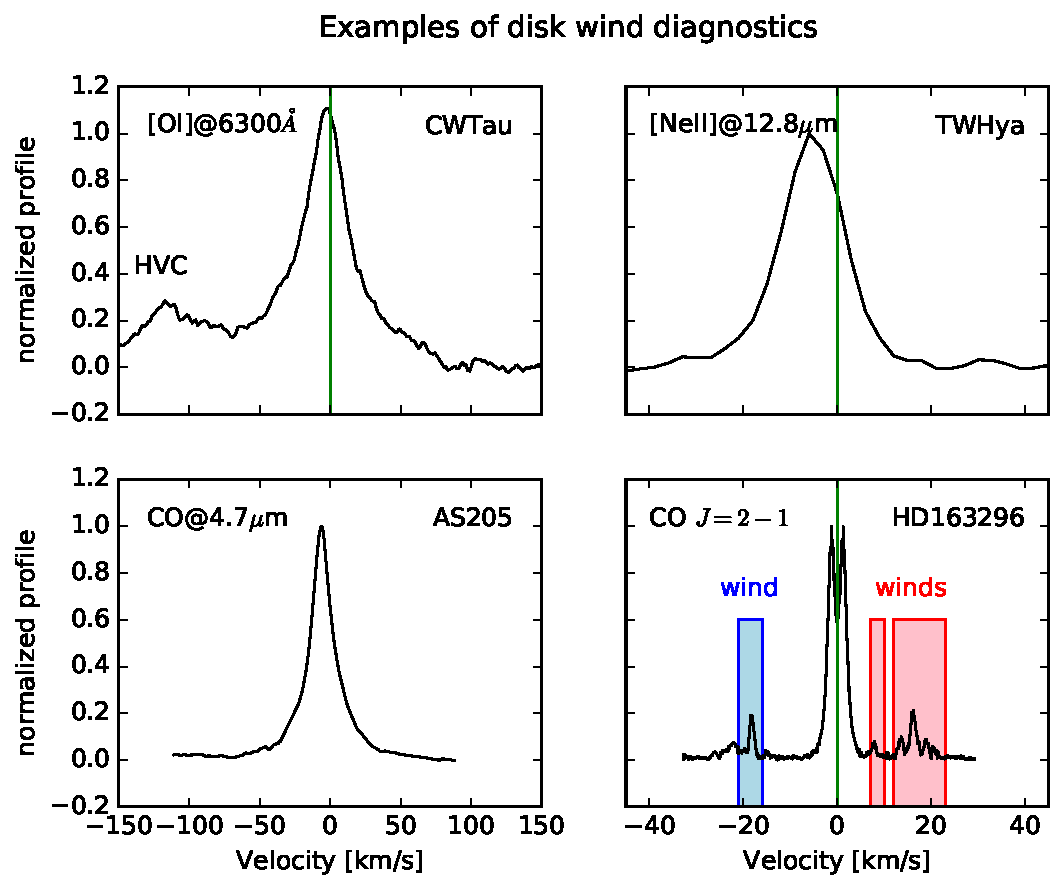
\includegraphics[width=0.7\textwidth]{winds.pdf}

   \caption{Examples of wind diagnostics. The [OI] 6300 Å profile of CW Tau is from Simon et al.\ (2016), note that the highvelocity
component (HVC) is associated with fast jets. The [OI] 5577 Å transition is weaker than the 6300Å but shows a
very similar low-velocity profile (Simon et al.\ 2016). The CO-M band profile of AS205 is from stacked CO rovibrational
lines around 4.7$\mu$m (Banzatti \& Pontopidan 2015). The [NeII] 12.8$\mu$m profile is the mean profile from Pascucci et al.
(2011) and the CO J=2-1 profile of HD163296 is from Klaassen et al.\ (2013). All profiles, except that of AS205, are in
the stellocentrc reference frame. Emission shifted in velocity with respect to the stellar velocity is indicative of unbound
gas. M-band CO profiles do not have an absolute velocity calibration, indication of a slow wind in AS205 comes from
spectro-astrometry (Pontoppidan et al.\ 2011). This figure is
taken from an upcoming review on transition disks by Ercolano \& Pascucci (2017, to appear in Royal
Society Open Science).}
              \label{fig:lines}%
    \end{figure}

A number of disk wind tracers have been studied to date, both
observationally and theoretically. To date however no diagnostic could
be identified to directly measure the wind properties. 
Figure~\ref{fig:lines}, taken from an upcoming review on transition disks by
Ercolano \& Pascucci (2017, to appear in Royal Society Open Science)
shows an example of possible wind diagnostics, which are summarised in
the caption.  

We will divide our discussion on wind diagnostics into two parts,
ionic and atomic species on the one hand and molecular species on the
other. 

\vspace{0.5em}{\Tcol\bf Ionic and atomic species}\\
The presence of disk winds has been confirmed via the
observation of a few km/sec blue-shift in the line profiles of a
number of tracers like [NeII]~12.8$\mu$m and [OI] 6300 (e.g.\ Pascucci
et al 2007, Rigliaco et al.\ 2013) and a number of collisionally excited lines in the optical
region (Natta et al.\ 2014). 

 \begin{figure}
   \centering
   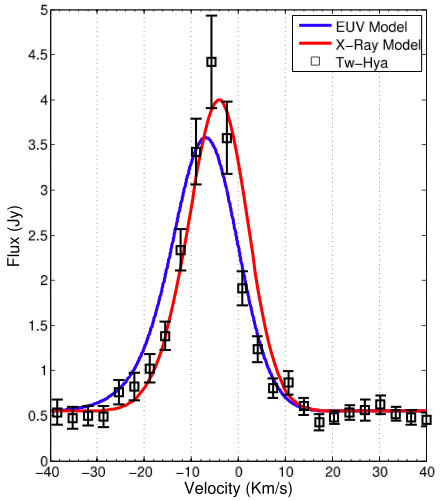
\includegraphics[width=0.5\textwidth]{neii.jpg}
   \caption{NeII 12.8$\mu$m line profile as predicted by the X-ray
     models of Ercolano \& Owen (2010), red line, and  by the EUV-only
     model of Alexander (2008), blue line, compared to the observation
     of TW-Hya by Pascucci et al.\ (2009), black line.
}
              \label{fig:neii}%
    \end{figure}

We have demonstrated, however, that the  [NeII]~12.8$\mu$m and the
optical forbidden lines 
cannot be used to infer the underlying 
mass-loss-rates (e.g.\ Ercolano \& Owen 2010, Ercolano \& Owen 2016). 
 For example, the intensity and the profile of the [NeII]~12.8$\mu$m line
 can be equally well fitted using an EUV (Alexander 2008) or an X-ray
 photoevaporation model (Ercolano \& Owen 2010), as shown in
 Figure~\ref{fig:neii}. The problem with the 
 [NeII] line is that the Ne+ formation route can occur both via the
 removal of a valence electron in the fully-ionised winds driven by
 EUV radiation, but also by charge exchange of Ne++ with neutral H
 which is abundant in the quasi-neutral winds driven by X-ray. 
The problem with the [OI] 6300 line and all other optical collisionally
excited lines considered to date is the strong temperature dependence
imposed by the Boltzmann term in the emissivity. This means that these
lines are mostly just tracing the hot layer of the wind heated by the
EUV radiation and not actually tracing the bulk of the wind where it
matters (Ercolano \& Owen 2016), hence they
cannot be used to infer mass-loss-rates or to constrain the wind
driving mechanism.   

This picture was further complicated by the recent high spectral
resolution observations of  Simon et al.\ (2016)  who found that low velocity
emission in [OI] forbidden lines, classically attributed to a
slow-moving disk wind, is present in all T-Tauri stars with
dust disks, even those classified as WTTs, but it is best fit
by a superposition of a broad and a narrow component. 
Most of the broad component emission
arises within 0.5AU and Simon et al.\ (2016) interpret it
as being produced in a magnetically driven wind, given that the
emitting region is well inside the gravitational 
potential well 
of the central star. The narrow component, which, unlike the broad
component, is always present in also in transition
disks, traces gas further away (0.5-5 AU) and is probably associated
with photoevaporative winds.

The interpretation of the broad component as a tracer of a magnetic
wind is however problematic for a number of reasons. The main problem
is that one would need a very large scale height to overcome the fact
that the emitting volume dominates as one goes to larger
radius. Presumably a very large magnetic pressure would be needed to
achieve this. Furthermore, if an hypothetical magnetic wind would
have enough density to match the observed broad component, it may also absorb
out all UV flux, which would then not be available to irradiate the
wind at larger radii, hence being at odds with the observation of the
narrow line component. 

 \begin{figure}
   \centering
   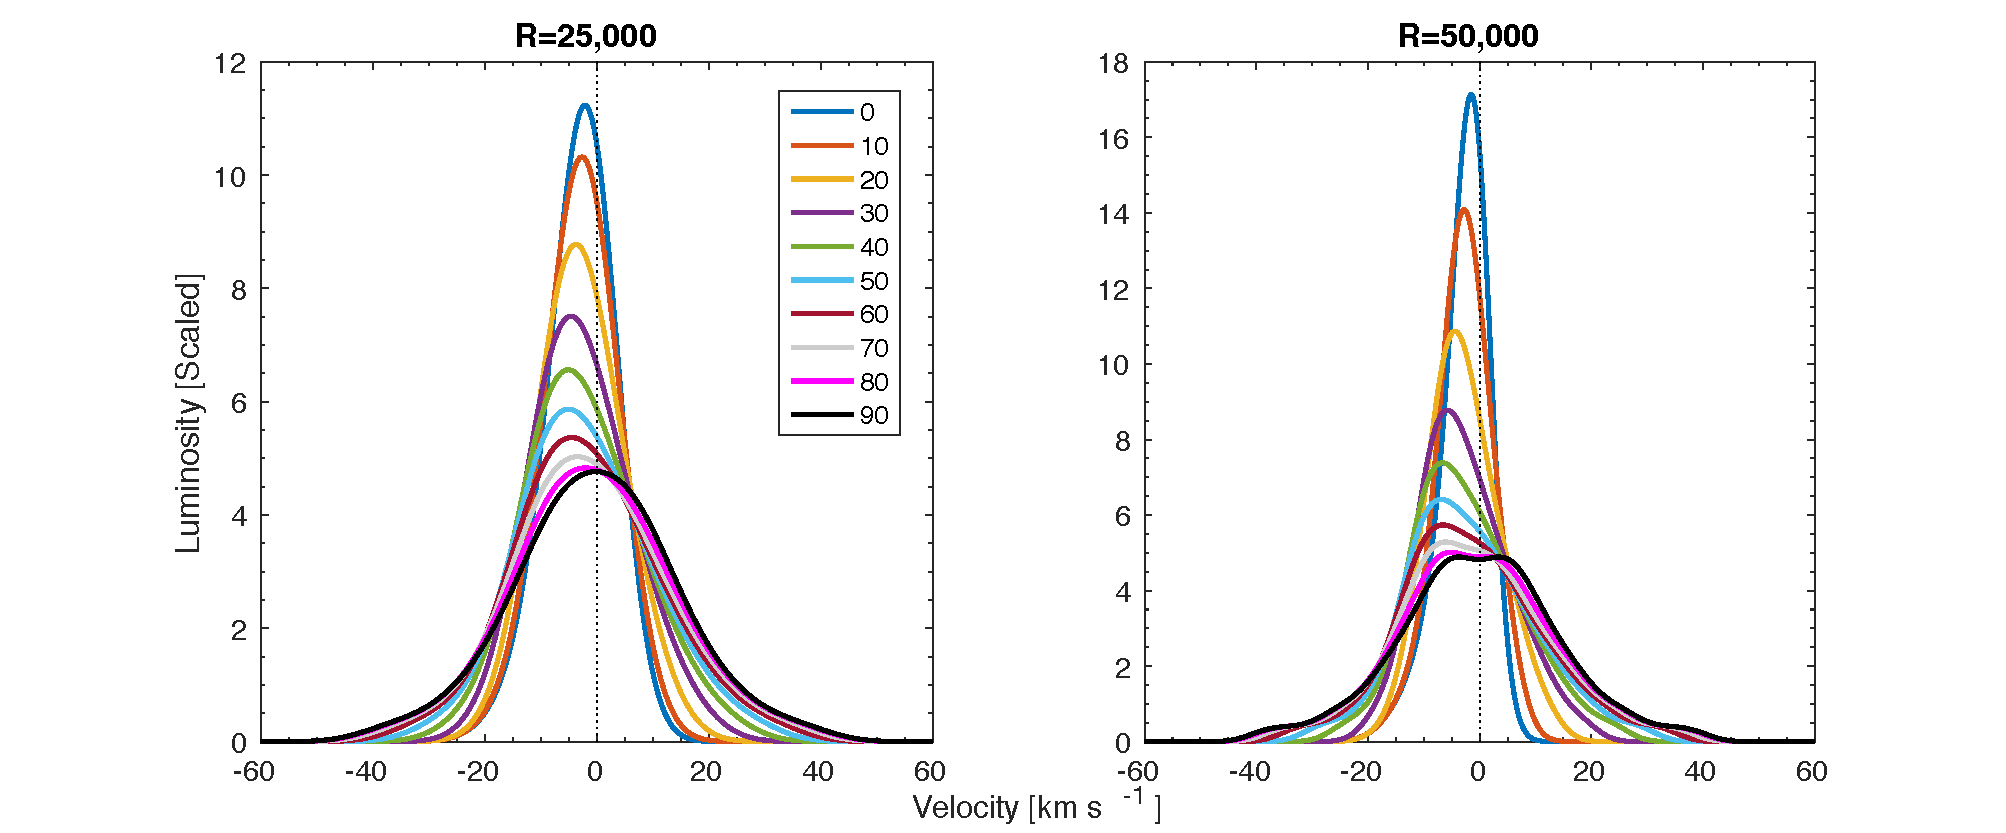
\includegraphics[width=0.97\textwidth]{lines_both.pdf}
  
   \caption{[OI] 6300 line
profiles for the high resolution hydrodynamical calculations of
Ercolano \& Owen (2016) for R=25000 (\caphighlight{left panel}), 
which represent the resolution of the
Rigliaco et al (2013) data, when the two component had not been
resolved yet, and R=50000 (\caphighlight{right panel}, which is more representative
of the work of Simon et al.\ (2016). In the left panel wings due to the
bound material are clearly seen, but they are much smaller than those
presented by Simon et al.\ (2016).
}
              \label{fig:wings}
    \end{figure}


An alternative explanation could be that the broad
component is not produced in the wind, but is emitted by bound
material in the disk itself. The broad component, if coming from the
inner disk, cannot have however a thermal origin. We have tested that
with a new higher resolution set of hydrodynamical calculations,
similar to those presented by Ercolano \& Owen (2016), which
extend further into the inner disk, to $r_{\rm in}$=0.04~AU. The line
profiles for the high resolution hydrodynamical calculations are shown
in Figure~\ref{fig:wings} for R=25000, which represent the resolution of the
Rigliaco et al (2013) data, when the two component had not been
resolved yet, and R=50000, which is more representative
of the work of Simon et al.\ (2016). The
R=50000 line profiles in our simulations do show broad wings at high disk
inclinations. The wings are due to bound material in the inner
disk. However the wings from our high resolution models are still much
smaller (i.e.\ do not carry enough flux) than those detected by
Simon et al.\ (2016). In fact in our calculations the line flux
is completely dominated by the (unbound) emission at larger
radii. This is easy to understand as the flux is proportional to
density squared times the volume and the volume for an isothermal
region in the disk scales like R$^{7/2}$ ($R^2\times H$). Given that
the density does not fall off steeply enough in the heated region then
the emission at larger radii dominates. For 
example a density profile set by the absorption of photons to a fixed
column - indicative of our case - would fall of approximately as
$n\propto1/R$, provided the absorption is dominated at large radius.

Our calculations show nevertheless that bound material in the very
inner disk can indeed produce broad wings. If the column of emitting
bound material were larger then stronger wings would be produced. A
non-thermal process acting at higher columns in the inner disk, as for
example dissociation of the OH molecule, could
indeed produce the missing flux in the wings. This could also be
blue-shifted if the OH-layer extends to the base of the wind (see e.g.
Gorti et al.\ 2011). As our codes currently
lack chemistry we have been unable to test a non thermal
origin of the broad component. This is however an important task, as
if confirmed, there would be no need to invoke magnetic disk winds to
explain the observations.  

 While a number of chemical models exist
of the deeper, denser regions of disks, no model is currently
available for the optically thinner disk winds. The work of Gorti, Dullemond \&
Hollenbach (2009), while carrying out detailed chemical calculations
extending to the disk atmosphere, used a hydro{\it static} disk model which
was analysed in a 1+1D fashion. Without hydro{\it dynamics} no predictions
on line profiles can be made.  
Studying the kinematic of the emitting gas is the only way to
constrain the origin and intensity of the disk wind and hence shed
light on the driving mechanism behind the dispersal of disks and the
formation of Type 1 transition disks. 

\vspace{0.5em}{\Tcol\bf Molecular species}\\
Mid-infrared observations of molecular lines (e.g.\ CO) provide a new
promising alternative to directly measure disk winds. Indeed recent
observations suggest that these lines may be tracing a disk wind which
is slow and partially molecular (e.g.\ Pontoppidan et al.\ 2011; Brown et al.\ 2013). 
The spectro-astrometric survey of molecular gas in the inner regions of
protoplanetary disks using CRIRES, the high-resolution infrared
imaging spectrometer on the Very Large Telescope (Pontoppidan et
al. 2011), showed that for several sources the astrometric signatures
are dominated by gas with strong non-Keplerian (radial) motions. These
authors concluded that the non-Keplerian spectro-astrometric
signatures are likely indicative of the presence of wide-angle disk
winds. 
More observations of this type are planned after the update of
the CRIRES instrument, which is expected to be completed by
2019. Observations with ALMA in molecular lines like e.g.\ CO J = 2-1
and J = 3-2 emission are also able to trace the presence of a wind (e.g.Klaassen et al.\ 2013, 2016).  
Molecular lines are sensitive to the mass loss rates since they
sample a significant area of the wind launching regions. However the
exploitation of molecular tracers is currently severely hampered by
the lack of a suitable hydrodynamic wind model coupled to chemistry
and to dust evolution models (which dominate the opacity in the wind)
to interpret the observations.

Molecular tracers of outflow activity are common in the protostellar
phase, they also probe a low velocity ($<$10\,km/s) component whose
intensity decreases while the opening angle increases going from the
Class~0 through to the Class~II phase (e.g.\ Frank et al.\ 2014 for a
recent review). This slow wide-angle component, around a much faster
jet, is naturally produced in MHD disk winds launched out to several
AU (e.g.\ Pudritz et al.\ 2007, Panoglou et al.\ 2012). ALMA maps of
outflow activity are corroborating this picture by providing the
sensitivity to study in detail the faint Class~II sources, see
e.g.\ the CO disk wind surrounding the fast jet from the
$\sim$4\,Myr-old Herbig~Ae star HD~163296 (Klaassen et
al. 2013). Interestingly, the rough mass loss rate from the molecular
wind is inferred to be similar to the mass accretion rate onto
HD~163296 suggesting that winds contribute significantly to disk
dispersal. Like optical forbidden lines, M-band CO ro-vibrational
lines also show a broad and a narrow line emitting region
(e.g.\ Banzatti et al.\ 2015) with FWHMs typically larger than the [OI]
6300\,\AA{} lines suggesting emitting gas closer to the central star
(Simon et al.\ 2016). Blueshifts of $\sim$5\,km/s are reported in 4 out
of  7 single-peaked CO lines (Bast et al.\ 2011) while clear evidence
of non-Keplerian motion is found in 2 out of the 16 sources observed
with the spectro-astrometry technique (RU~Lup and AS~205N, Pontoppidan
et al.\ 2011). In the case of AS~205N, followup high-resolution ALMA
observations also show deviations from Keplerian rotation in mm CO
emission which could be due to a low velocity disk wind or tidal
stripping by its companion AS~205S. 

It is thus of outmost importance to understand how to distinguish the
outflow signatures of a photoevaporating wind from those of a wide
angle magnetically driven wind. Spectral line profiles are in this
case helpful to determine the spatial location of the outflow, or of
the region where the line originates. Comparison of profiles from
transition disks and primordial disks are very helpful to shed light
of the wind driving mechanism at different times. Indeed Ercolano \&
Owen (2010, 2016) and Simon et al.\ (2016) both discuss the expected
and observed differences in the two cases. In general, a profile which
shows a large component coming from unbound material at small disk
radii ($<0.5$AU), for example is difficult to explain in terms of
photoevaporation, where mass loss is only expected outside the
so-called gravitational radius ($>$0.5AU), while, classically,
magnetically driven wide angle winds are expected to come from the
regions closer to the star. 


\subsection{Contributions of the team to the study of disk chemistry and ionisation}
The study of chemistry in disk winds self-consistently with their
atmospheres is pretty much uncharted territory, this also contributes
to the fact that the determination of the ionisation level in disks is
still based on simple models (e.g.\ Perez-Becker \& Chiang, 2011). The
team members have collectively large expertise in chemical and ionisation
calculations of various environments including disks interiors as well
as expertise in the development of photoevaporation models. This puts
them in a prime position to be able to pioneer this work. The
contributions of the PI Ercolano to the field of photoevaporatve winds
can be appreciated from the work described in the previous section. In what
follows, we briefly describe the state-of-the-art in the field of disk
chemistry and ionisation, where the other team members of Project B2 have played
an important role.  

\vspace{0.5em}\noindent{\Tcol\bf Chemical models of protoplanetary disks}\\
Gas and solid chemistry play a key role in the evolution of planet-forming disks and in planet formation theories, and determine the original composition of (exo)-planets (Henning \& Semenov 2013).  Planets are formed in protoplanetary disks that evolve over typical lifetimes of a few millions years (Fedele et al.\ 2010) by viscous spreading (e.g., Hueso \& Guillot 2005; Bailli$\acute{\textsf e}$ \& Charnoz 2014) combined with photoevaporation (Alexander et al.\ 2013). During that time, the dust grains coagulate to each other to reach the size of meter- then kilometre- sized bodies (Birnstiel et al.\ 2010, 2012). Those bodies can agglomerate into planets or participate to the late episodes of heavy bombardments, bringing material onto planetary atmospheres and surfaces. Detection of the main belt asteroids reinforces the idea that asteroids may have brought most of the water on Earth (Jewitt 2012). Another key role played by chemistry is to set the location of the disk region where water is frozen onto solids, the so-called ice zone. Beyond the water ice zone, giant gas planets like Jupiter can form after the rapid accumulation of solid cores of 10 Earth masses by the core-accretion model (Helled et al.\ 2014, $\ddot{\textsf O}$berg et al.\ 2015a, Helling et al.\ 2014).

Contrary to their young counterpart 'hot-corinos' (Cazaux et al.\ 2003), a much limited amount of molecules have been detected in protoplanetary disks. The outer disk molecular inventory includes CO, CN, HCN, formaldehyde, C$_2$H, CS, CH$_3$CN, HCO$^+$ and after a lot of effort CH$_3$OH (e.g.\ Dutrey et al.\ 2014;  $\ddot{\textsf O}$berg et al.\ 2015b; Walsh et al.\ 2016). The low abundance of many of the molecules has been ascribed to a combination of photodissociation at the disk surfaces and freeze-out onto grain surfaces towards the disk mid-plane. Simple molecules such as H$_2$, HD, CO, CO$_2$, H$_2$O, C$_2$H$_2$, HCN, N$_2$H$^+$, and potentially CH$_3$OH, have been detected from the terrestrial planet-forming region of protoplanetary disks by high-resolution spectrometers from ground-telescopes and by the Spitzer Space Telescopes (Pontoppidan et al.\ 2014). The gas is sufficiently warm such that many molecules are formed by neutral-neutral reactions with activation barrier. The ro-vibrational transitions in the mid-infrared have the advantage that homonuclear species such as CO$_2$ or C$_2$H$_2$ can emit contrary to pure rotational transitions. In addition to those small species, Polycyclic Aromatic Hydrocarbons (PAHs) infrared emissions are prominently seen from disks around the UV-luminous Herbig Ae stars. 

Carbonaceous compounds such as tholins may have been detected in an evolved disk (Debes et al.\ 2008, K$\ddot{\textsf o}$hler et al.\ 2008). The detected lines in both the inner and outer disk are emitted well above the mid-plane. Although the amount of detected species may be low, the chemical paths are not because of the large range of density, temperature, and UV field strength. Thermo-chemical disk models use a common unique network to model the entire disk. Many questions remain on the origin and survivability of complex organic molecules in protoplanetary disks in general and in the Solar Nebula in particular. We expect that grain surface thermal- and photoreactions (UV and X-ray) and high-energy particles play an important role in the formation of complex species in the disk regions where water can be frozen onto grains (Throop 2011, Ciesla \& Sandford 2012, Walsh et al.\ 2014). The energetic radiation break molecular bonds producing reactive radicals and ions but stellar wind can inhibit the propagation of cosmic rays (Cleeves et al.\ 2013). Grain surfaces enhance considerably the probability for two species to meet and form other species. Throop (2011) and Ciesla \& Sandford (2012) models do quantify neither the specific species that are synthesised nor their amount, but have demonstrated that complex organics can indeed form on the Solar Nebula grain surfaces. In addition Ciesla \& Sandford (2012) results suggest that gas and dust transport in the Solar Nebula (and in disks) will interconnect disk regions with dissimilar physical and chemical environments.

Members of the PI group are active collaborators within the ProDiMo\footnote{http://homepage.univie.ac.at/peter.woitke/ProDiMo.html} consortium (see e.g.\ Thi et al.\ 2014; Woitke et al.\ 2016).  ProDiMo is a software package to model static protoplanetary disks including gas phase, X-ray and UV-photo-chemistry, gas heating and cooling balance, disk structure and (dust \& line) radiative transfer. Surface chemistry has been recently included (Thi et al., in preparation).
%Understanding protoplanetary disk evolution is one of the major endeavours in astrophysics. All studies are based on the alpha viscous-disk theory, which drives the disk spreading (Lynden-Bell \& Pringle 1974). The main contender to explain the viscosity is the Magneto-Rotational Instability (MRI), which efficiency alpha depends on the ionisation of the gas (Armitage 2011). Previous studies did assume a temporarily and spatially constant value for the efficiency alpha, although recent works already include the effect of gas heating by absorption of the stellar radiation (Bailli$\acute{\textsf e}$ \& Charnoz 2014). A realistic disk evolutionary model would require the detailed computation of the chemistry and hence of the gas ionisation at each location of the disk over the discユs lifetime. The efficiency of the MRI is strongly related to the strength of the different couplings between the charge carriers and the neutral gas in the disks (Ohm resistivity), or between the ions and the electrons (Ambipolar diffusion). Knowledge of the disk chemistry in general, and of the ionisation fraction in particular is paramount (Bai 2011). The charge carriers in disks are either electrons, atomic and molecular ions, polycyclic aromatic hydrocarbons (PAHs) or dust grains. The abundances of the carriers vary throughout the disk due to ionisation processes (photoionisation by UV and X-ray photons, cosmic-rays), recombination with electron, and charge exchanges. The rates of these processes are functions of the gas composition, the gas and dust temperatures, and the UV and X-ray fluxes inside the disks. Therefore the computations of the abundances require a detailed gas and dust physics and chemistry modelling together with continuum and line radiative-transfer. The ionisation fraction will affect the viscous evolution of the disk density structure, which in turn will affect the chemistry. Disks can also lose mass by photoevaporation at its surfaces due to illumination by the central star or by nearby OB stars (Alexander et al.\ 2014).

\vspace{0.5em}\noindent{\Tcol\bf Ionisation in disks}\\
An accurate calculation of ionisation-recombination balance in dense protoplanetary conditions is essential for
understanding various fundamental problems, such as coupling of the gas with magnetic field (Li et al.\ 2014), accretion
processes (Turner et al.\ 2014), chemistry (Semenov et al.\ 2004; Larsson et al.\ 2012) and dust evolution (Okuzumi et al.\ 2011b; Akimkin 2015). The charging of grains in such environments affects their interaction of surrounding ions and electrons
(Okuzumi 2009; Weingartner \& Draine 1999) and hence modifies the chemistry at the grain surface.

Both the ionisation and recombination processes can arise from several sources. Primary agents of ionisation in dense gas
(at visual extinctions above $A_{\rm V}\sim 10-30$\,mag, where interstellar UV photons are absorbed) are X-rays, cosmic-rays (CRs), and the decay of radionuclides, leading to the ionisation fraction that decreases with density (Oppenheimer \& Dalgarno 1974; Caselli et al.\ 2002; Maret et al.\ 2006). In disks around young, active stars the situation is complicated due to the presence of stellar X-rays (Glassgold et al.\ 1997) and the possible exclusion of low-energy CRs by protostellar winds (Cleeves et al.\ 2013b). Efficiency of stellar X-rays to ionize the circumstellar gas depends on the total fluxes and the hardness of the spectra (Igea \& Glassgold 1999; Ercolano \& Glassold 2013). Near the disk midplane, where X-rays and CRs are strongly attenuated, radioactive elements may substantially contribute to the electron fraction. In this case the ionisation rate is proportional to the abundance of the radioactive element and its decay rate (Umebayashi \& Nakano 2009; Cleeves et al.\ 2013a): Short-lived radionuclides (SLR, mostly $^{26}$Al with half-life $7.4\times 10^5$~yr) contribute comparatively more than long-lived radionuclides (LLR, mostly $^{40}$K with half-life $1.3\times 10^9$~yr), but decay faster.

While the treatment of ionisation, despite the variety of ionisation sources, could be reduced to a single (total)
ionisation rate, the description of recombination is less straightforward. At sufficiently high densities, where the
dominant sink of free electrons and ions are dust grains, the recombination rate non-trivially depends on properties of the
grains (Okuzumi et al.\ 2011a,b; Ivlev et al.\ 2016).

The grain charges are determined by different mechanisms operating in different regions of disks: In the disk atmosphere, the
photoelectric emission from grains is a prominent charging mechanism, leading to positive charges (Weingartner \& Draine 2001; Weingartner et al.\ 2006; Akimkin 2015). Not only stellar radiation, but also H$_2$ fluorescence induced by CRs can contribute to this (Ivlev et al.\ 2015). In the inner, midplane disk regions the photoemission becomes negligible, and the grain charges are determined by collection of electrons and ions from the surrounding weakly ionized gas, leading on average to negative grain charges.

Depletion of electrons in dense disk regions, caused by the presence of negatively charged grains, significantly reduces the
degree of ionisation (Umebayashi 1983; Umebayashi \& Nakano 1990; Nishi et al.\ 1991). As the ionisation controls the coupling of the gas to the magnetic field, and hence the development of the magnetorotational instability (MRI, e.g.\ Velikhov 1959, Balbus \& Hawley 1991; Armitage 2015), dust is the essential ingredient for any MRI model. It has been shown that the grain size critically affects the size of a disk's ``dead zone'' (Sano et al.\ 2000; Salmeron \& Wardle 2008; Bai 2011a,b; Dudorov \& Khaibrakhmanov 2014).

Recently we have developed an exact analytical model which describes ionisation and dust charging in dense disk conditions,
for arbitrary grain-size distribution (Ivlev et al.\ 2016). Unlike previously developed approaches (Ilgner \& Nelson 2006; Okuzumi 2009; Fujii et al.\ 2011; Dzyurkevich et al.\ 2013; Mori \& Okuzumi 2016), our model does not make assumptions on the form of the grain charge distribution, and enables convenient analysis of results in a general form, in terms of a few dimensionless numbers, which allows us to identify universality in the behavior of the charged species.


\subsection{Project-related publications}
%
% Please list your own publications related to the proposed project, 
% adhering to the rules of the DFG guidelines 1.91. In brief, please note: 
% - Up to 10 publications
% - The work must be published or accepted.
% - Publications on astro-ph (arXive, SPIRES or articles with a DOI) count as published. 
% - Any work that is only in the status ``accepted'' MUST be attached to the proposal
%    together with the acceptance letter.
% - All publications in this section CAN be attached to the proposal. Please limit these
%    attachments to a minimum and please note that the reviewers may not read the attachments -
%    the proposal has to speak for itself.
% - The number of allowed publications refers to the sum of the publications listed
%    in ``1.1.1 Articles published or officially accepted by publication outlets...'' and 
%    in ``1.1.2 Other publications''. Publications which only exist on public repositories 
%    belong into the category ``Other Publications''.
%

\begin{literature}

\item \textbf{Caselli P.}, Walmsley C.M., Terzieva R., Herbst
  E. \textit{The ionization fraction in dense cloud cores}, 1998, ApJ,
  499, 234. In this work we run chemical models and compared the
  results with observations to estimate the ionisation fraction and
  the cosmic ray ionisation rate for the first time in a statistically
  significant sample of dense cloud cores. These results have been
  used in recent theoretical work dealing with the propagation of
  cosmic rays in molecular clouds. The techniques developed in this
  papers will be useful to assess the ionisation structure of disks.

\item \textbf{Caselli P.}, Walmsley C.M., Zucconi A., Tafalla M.,
  Dore L., Myers P.C. \textit{Molecular Ions in L1544. II. The
    Ionization Degree}, 2002, ApJ, 565, 344. We measure for the first
  time the ionisation fraction across a contracting low-mass dense
  cloud core with the help of a simple chemical network and comparison
  with observations of CO and protonated as well as deuteronated
  N2. Low ionisation fractions (1e-9) are predicted toward the core
  center, with a consequently short ambipolar diffusion time scale
  (comparable to the free-fall time scale). The techniques developed in this
  papers will be useful to assess the ionisation structure of disks
  and the relevance of non-ideal magnetohydrodynamics regimes. 

 \item Keto E., \textbf{Caselli P.}, Rawlings J. \textit{The dynamics
     of collapsing cores and star formation}, 2015, MNRAS, 446,
   3731. We construct a reduced chemical network for oxygen chemistry
   (including water and carbon monoxyde), include it into a
   hydrodynamical code of the evolution of Bonnor-Ebert (BE) spheres
   and compare the results with observations.  For the first time, we
   demonstrate that dense cloud cores contract as unstable
   quasi-equilibrium BE spheres, while the singular isothermal sphere
   and Larson-Penston solutions for dense core contraction do not
   reproduce the observed line profiles.  This was only
   computationally possible
   because the number of reactions was reduced to the core. A similar
   approach will be used in B1. 

\item \textbf{Ercolano, B}. \& Glassgold, A.E. {\em X-ray ionization rates in
    protoplanetary disks}, 2013, MNRAS, 436, 3446. In this paper we
  calculate the ionisation rate in protoplanetary disks using our
  MOCASSIN photoionisation and radiative transfer code and a realistic
  X-ray ionisation spectrum. The rates
  developed here are becoming the new standard for inclusion in
  chemical codes and for the calculation of dead-zones and magnetic
  coupling within protoplanetary disks. This paper represent the new
  state-of-the-art after the widely used Igea \& Glassgold (1999)
  paper. 

\item \textbf{Ercolano, B.},  Drake, J.; Raymond, J., Clarke, C.
  \textit{X-Ray-Irradiated Protoplanetary Disk Atmospheres. I. Predicted Emission-Line Spectrum and Photoevaporation}, 2008, ApJ
  688, 398. In this paper we use the MOCASSIN code to present a first
  estimate of the magnitude of the X-ray photoevaporation process in
  protoplanetary disks. We obtain significant mass loss rates, showing
  the relevance of this process to the dispersal of disks. Before this work the
  importance of X-ray photoevaporation had not been recognised.  

\item \textbf{Ercolano, B.}, Clarke, C., Drake, J. \textit{X-Ray
    Irradiated Protoplanetary Disk Atmospheres. II. Predictions from
    Models in Hydrostatic Equilibrium}, 2009, ApJ 699, 1639. We
  further develop our models to include the feedback of X-ray heating
  on the disk-structure in hydrostatic equilibrium, and obtain more
  accurate estimates of the photoevaporation rates, which confirm our
  previous conclusions that the X-ray photoevaporation process is a
  main player in the dispersal of disks. These calculations form the
  starting conditions for the full hydrodynamical investigations to
  Owen et al. (2010). 

\item \textbf{Ercolano B.}, Owen J. {\em Theoretical spectra of
    photoevaporating protoplanetary disks: an atlas of atomic and
    low-ionization emission lines}, 2010, MNRAS 406,1553. We postprocess the
  models of Owen et al. (2010) and obtain synthetic observations of
  atomic and low-ionisation emission lines to be compared with the
  observations. We show that our models compare favourably with the
  observations available at the time.

\item \textbf{Ercolano B.}, Owen J.  {\em Blueshifted [O I] lines from
    protoplanetary disks: the smoking gun of X-ray photoevaporation},
  2016, MNRAS 460. 3472
  We produce new synthetic observations of a particularly promising
  diagnostic, and demonstrate that the observations available at the
  time (before Simon et al. 2016) are consistent with the
  photoevaporation model. We show however that this line cannot be
  used to measure mass-loss-rates and suggest that a thermochemical
  model of the wind launching region is necessary. 

\item \textbf{Ivlev, A. V.}, Padovani, M., Galli, D., \textbf{Caselli,
    P.} \textit{Interstellar dust charging in dense molecular clouds:
    cosmic ray effects}, 2015, ApJ, 812,135. We calculate the dust
  charging in the atmosphere of protoplanetary disks and dense
  molecular clouds, showing that cosmic rays often provide a dominant
  contribution due to the locally generated UV field. This hitherto
  completely neglected charging mechanism is expected to critically
  affect the dust evolution in the disks. 
 
\item \textbf{Ivlev, A. V.}, Akimkin, V., \textbf{Caselli, P.}
  \textit{Ionization and dust charging in protoplanetary disks}, 2016,
  to be published in ApJ. We develop an analytical model of ionization
  in protoplanetary disks. For a broad range of parameters and
  arbitrary grain size distributions, this enables self-consistent
  calculation of densities of the charged species and of the dust
  charges. The model can be easily included in available numerical
  codes following the dust evolution. 


\end{literature}

% \subsubsection{
% Articles published or officially accepted by publication outlets with scientific quality assurance;
% book publications}
% 
% \subsubsection{Other publications}
% 
% None
% 
% \subsubsection{Patents}
% 
% \paragraph{Pending}
% 
% None 
% 
% \paragraph{Issued}
% 
% None 

\section{Objectives and work programme}
\renewcommand{\leftmark}{\sc Objectives and work programme}

\subsection{Anticipated total duration of the project}

36 months

\subsection{Objectives}

\connect{The overarching aim of this project is together with projects B1 and C2 to quantitatively characterise the dispersal mechanism of protoplanetary disks, leading to the formation of Type 1 Transition Disks}. This will constrain the physical and chemical properties in the disk at the time of planet formation and provide case-specific limits to the timescales of formation and migration of gas giants, which must occur in a gaseous disks. 

The intermediate goals that will lead to the achievement of the project main aim are: 

\begin{enumerate}

\item Devise a chemical model appropriate for photoevaporative wind conditions which takes into account of the varying dust properties in the wind. 
\item Directly measure the wind mass-loss-rates and profiles by
  comparing synthetic line profiles from the models to existing and upcoming observations.
\item Devise a chemical/ionisation model appropriate for
  protoplanetary disk atmospheres that self-consistently accounts for
  the shielding of stellar radiation from the wind. This will allow to
  assess the role of magnetic fields for launching a wind.
\end{enumerate}

\subsection{Work programme including proposed research methods}
% for each applicant

 \begin{figure}
   \centering
   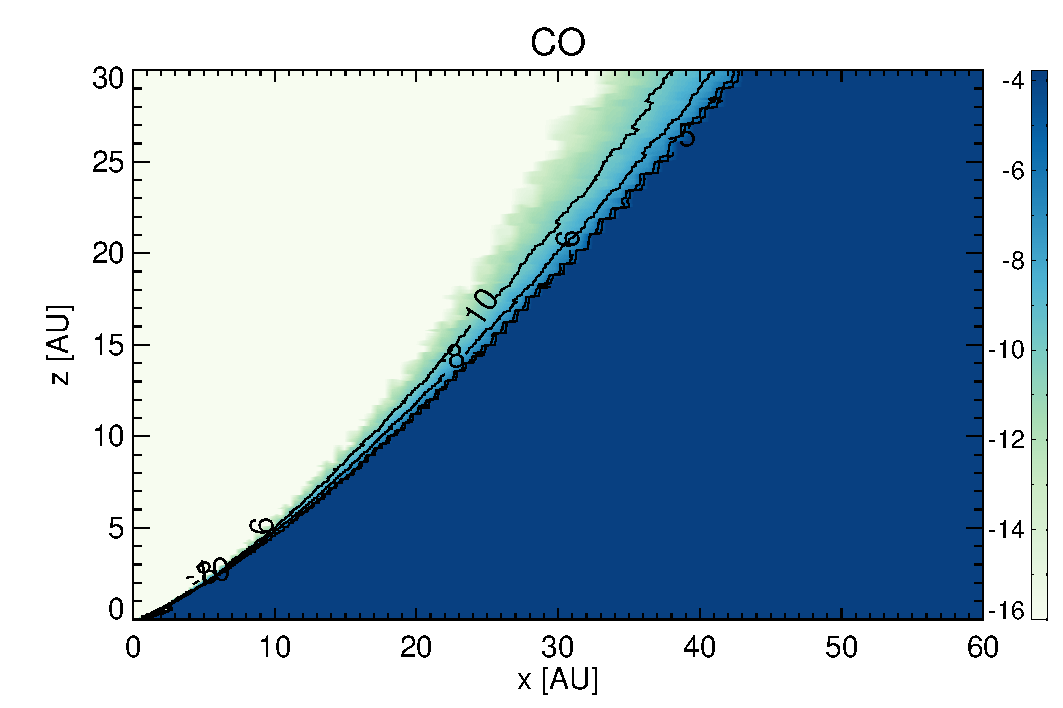
\includegraphics[width=0.47\textwidth]{Lx_2e29_CO.pdf}
   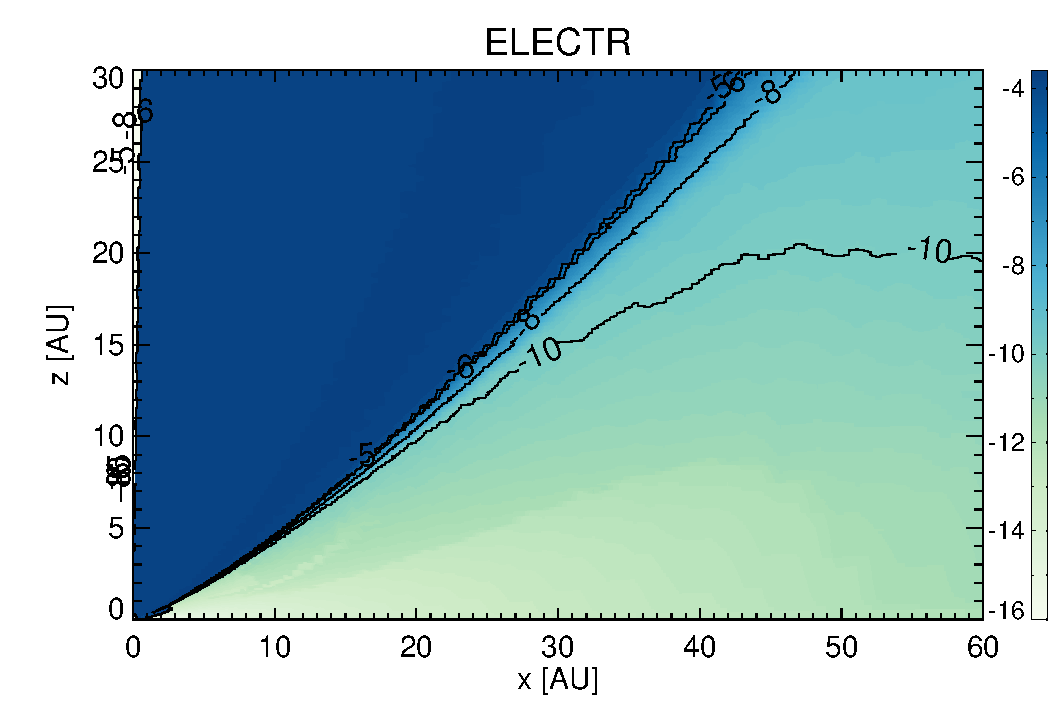
\includegraphics[width=0.47\textwidth]{Lx_2e29_ELECTR.pdf}
   \caption{CO (left) and e$^-$ maps from our toy chemical model
     applied to the Owen et al.\ (2010) wind solutions. See text for details
}
              \label{fig:chem}%
    \end{figure}


As will be detailed in what follows, a number of steps are required to
further develop our methods to be able to deal with the problem at
hand. Nevertheless as an example we have applied our chemical model to
the standard wind solution from Owen et
al. (2010). Figure~\ref{fig:chem} shows maps of the CO and of the
electrons resulting from our toy model. 


Some interesting features are already visible from this toy
calculation, most notably that CO survives in the atmosphere of the
disk and at the base of the wind, where it can be launched. 

We use now the simple calculation above to describe the limitations of
the current methods, which we aim to lift in this project. 

\begin{enumerate}
\item The model makes simple assumptions for the irradiating spectrum
of the central star (we assume here a radius and effective temperature
of 2.076~$R_s$ and 3862 K for the central star, which are appropriate
for a 0.7$M_{\odot}$ star at 1~Myr age, Baraffe et al.\ 1997, 2002).

\item Only thermal effects of X-rays on the gas
temperature are taken into account (i.e.\ the X-ray ionisation rate
to 0) and the current chemical network does not include specific
X-ray chemistry. 

\item A standard dust opacity model was used to attenuate
the FUV (Ossenkopf \& Henning, 1994). As the models depend strongly on
this a tailored dust model is necessary. 

\item The H$_2$ and CO self-shielding
calculation assumed constant 0.5 and 1e-4 abundances. This overestimates the true
shielding, so a more realistic model would need to iterate the
chemical model with updated shielding coefficient from the previous
iteration.

\item The chemical model is the KIDA 2015 release, which is a gas-phase
chemical network, but it takes the formation of H$_2$ on grain surface and
charge exchange with grains into account. The network however does not
include double or higher ionisation states, which would be produced by
X-rays. Freeze-out of gas phase species are also not considered, while
this is not a problem in the warm atmosphere and wind of the disk, it produces
unrealistically high CO abundance in the mid-plane. 

\item The chemical network is solved time-dependently, and evolved to 1 Myr,
which is longer than most of the chemical timescales at typical disk
densities (although this is not always true in the atmosphere). The
abundances shown are then roughly equilibrium abundances (especially since no
grains surface chemistry is considered). Time-dependence is likely to
play a role in the modeling of the tenuous disk atmospheres and
winds. 
\end{enumerate}

\subsubsection{Research tools and inputs}

The KIDA (http://kida.obs.u-bordeaux1.fr) code will be used as a
starting point, as this is continuously updated, based on new
experimental and theoretical work on rate coefficients.  From this, we
will extract a reduced network (as recently done in Kong, Caselli et
al. 2015 for the particular case of massive star forming regions),
where the chemistry of simple and abundant species such as CO, OH, O,
C, C+, … is followed with the same accuracy as with the more
comprehensive network.  We will then add important disk wind tracers
such as Ne, Ar and their ionised forms, as well as X-ray chemistry
based on work already described in the literature (e.g. Glassgold et
al. 2007; Meijerink et al. 2012; Akimkin et al. 2013).  

This chemical network will be inlcuded into the MOCASSIN+KROME, to solve the geometry independent radiative transfer through gas  and dust, including photoionisation and chemical calculation
  including X-rays. PI Ercolano has been working on coupling her 3D Monte Carlo photoionisation
and dust radiative transfer code MOCASSIN (Ercolano et al.\ 2003, 2005,
2008b) to the KROME package (Grassi et al.\ 2014), to perform arbitrary
chemical calculations (Ercolano \& Grassi, 2017, in
preparation). Simple photoionisation benchmarks from the set of
Pequignot et al.\ (2001) have already been successfully performed with
the new coupled version, and a toy network has also
been introduced, which is however inadequate for any realistic
modelling of disk chemistry. The development of an appropriate
chemical network to be included into MOCASSIN+KROME is indeed one of
the first tasks of the work program described below.

The advantage of using this new code compared to existing chemical
codes for disks, is that it allows a fully self-consistent treatment
of the radiative transfer and hence radiation field attenuation
through dust and gas. The code is fully 3D (but can work in 2D) and it
can handle complex, multi-component and space-varying dust grain models. 

MOCASSIN (without KROME) has already been used to post-process
hydrodynamical calculations of photoevaporating disks (e.g.\ Ercolano
\& Owen 2010, 2016) to produce synthetic spectral line profiles of
atomic and ionised species in the wind and atmosphere. 

The abundances calculated with MOCASSIN+KROME will then be further
post-processed using the popular RADMC-3D code, developed and mantained
by Prof.\ Dullemond (PI of project D2) or the MOLLIE (Keto et
al. 2004) or the LIME (Brinch \&
Hogerheijde 2010) codes, which have also already been used by members of our
B2 team for other projects. 


\subsubsection{Work Program}


The project will develop along a path of growing complexity. It is
possible that some of the tasks in the last stage (time-dependance)
may be carried over to the next funding period. While this complex
project will be led by the postdoc, the PIs and collaborators will
also take an active part in the work. One of the PIs of this project
has extensive experience in devising efficient and reliable reduced
networks (see e.g.\ Keto \& Caselli 2008, 2010; Keto, Rawlings \&
Caselli 2014), while one of the collaborators and the other PI are
leading effort in the ionisation structure and radiative transfer of
disks (e.g.\ Ivlev et al.\ 2016, Glassgold \& Ercolano 2013, Ercolano
et al.\ 2008,2009).   

\paragraph{Months 1-12}

\noindent {\Tcol\bf The reduced network.} A first task for this
project is to simplify the gas-grain chemistry by reducing the chemical network to the minimum number of reactions needed to properly follow the formation/destruction of important species (in particular Hydrogen, Carbon, Oxygen as well as simple C-, O-bearing molecules) and the electron abundance or ionisation fraction. 
The reduced chemical network will be benchmarked against comprehensive chemical networks to make sure that the abundances of  important (diagnostic) species such as C$^+$, C, O, CO are well reproduced in the range of conditions appropriate for evolved and
transitions disks. This will imply running the comprehensive and reduced networks in a grid of physical conditions by varying temperature, density, and UV/X-ray fluxes.  As lines of Ne ([NeII], [NeIII]) and Ar ([ArII]) are good tracers of disk winds (e.g.\ Pascucci 2007, Szul$\acute{\textsf a}$gyi et al.\ 2012), Ne and Ar will be included in the chemical code. 

Particular attention will be dedicated to the inclusion of X-rays and the identification of the regions within the disk where X-rays, FUV photons and cosmic-rays (CRs) dominate the chemical and thermal properties. Typical assumption is that the X-ray spectrum is given by the bremsstrahlung spectrum ($I_{\nu} \simeq 1/E \times exp(-E/kT)$ on the 0.1 - 10\,keV energy range (e.g.\ Glassgold et al.\ 2007, Aresu et al.\ 2011, Meijerink et al.\ 2012). The observed luminosity ranges are L$_X$ = 10$^{29} - 10^{31}$\,erg/s (based on the Taurus survey, G$\ddot{\textsf u}$del et al.\ 2007). The X-rays heat up the gas with 10-40\% efficiency (UV heating has only a few per cent efficiency). 

Impinging X-rays may ionise the disk or wind material via primary or secondary ionisation. Primary ionisation may produce a single or multiple electrons due to the Auger effect. Their energy range depends on the shell from which  the Auger electron originates. The rate coefficient is given by the integral of the product of the X-ray energy spectrum and the ionisation cross section of the element (see e.g.\ Meijerink 2012, equation A.13). Secondary electrons might have keV energies, capable of $\sim$20-30 hydrogen ionisation. In fact the secondary electron ionisation rate per H nucleus is higher than the primary by an order of a magnitude, thus often only the secondary ionisations are considered in chemical models (e.g.\ $\acute{\textsf A}$d$\acute{\textsf a}$mkovics et al.\ 2011, Bruderer 2012).
The exact expressions and the peak electronic ionisation cross sections are given in $\acute{\textsf A}$d$\acute{\textsf a}$mkovics et al.\ (2011). 

Chemical models in the literature deal differently with X-ray reactions. The Semenov et al.\ (2010) and associated papers (Akimkin et al.\ 2013) model these reactions as an additional contribution to cosmic ray ionisation reactions (i.e.\ the rate is given by $R = \alpha \times (\zeta_{CR} + \zeta_X)$). Bruderer et al.\ (2012) accounts for only the secondary ionisation. Finally, Meijerink et al.\ (2012) take both the primary and secondary ionisation into account, as described above (see also Table 3 in Henning \& Semenov 2013).

X-rays affect the chemistry in various ways: (i) X-rays might directly ionise H (while FUV radiation does not), initiating H$_2$ formation via the H-path. In high temperature regions, where the grain surface H$_2$ formation is less efficient, this reaction might contribute significantly to the total H$_2$ formation rate. (ii) Secondary electrons interacting with H$_2$ produce H$_2^+$ that quickly reacts with a further H$_2$ to form H$_3^+$ or reforms H$_2$ via charge transfer with neutral H. This can lead to H$_3^+$ abundances as high as 10$^{-8}$. This then initiates efficient ion-neutral reactions which e.g.\ result in efficient H$_2$O production (see e.g.\ Meijerink et al.\ 2012). Furthermore, the heating effect might also increase the rate of neutral-neutral reactions with reaction barriers. (iii) H$_3^+$ initiates ion-molecular reactions which keep molecular abundances high even at high temperatures (if X-rays are present, compares to only FUV). (iv)
Ne, Ne+, Ar and Ar+ have ionisation potentials 21.56, 40.96, 15.76 and 27.63\,eV respectively. They are only ionised due to X-rays or X-ray induced fast electrons. Therefore, their ionisation is an indicator for X-rays and, as already mentioned, these species will be included in our chemical models. (v) Enhanced CO destruction through reaction with He$^+$, which has an ionisation energy of 24.6 eV (CRs can also ionize it). (vi) Other observational tracers (suggested by Meijerink 2012) are: H$_2$O, Ne$^+$, C/C$^+$ ratio,O$^+$.

Finally, while X-rays are unlikely to interact at the low column densities of the wind they are crucial for the chemistry in the underlying disk material, which feeds the wind. 

\paragraph{ Months 13-18}

\noindent {\Tcol\bf Line diagnostics from chemical models.} Once the reduced network is benchmarked and tested, it will be included in the MOCASSIN-KROME code by the co-PI Ercolano. The MOCASSIN-KROME code will be used to obtain the chemical abundances, while, radiative transfer codes available at the PI Institute (RADMC-3D\footnote{http://www.ita.uni-heidelberg.de/~dullemond/software/radmc-3d/} and LIME\footnote{http://www.nbi.dk/~brinch/index.php?page=lime}) will be used to obtain fluxes in dust continuum and lines to then perform simulated observations and compare with available data and/or make predictions for future observations. We note that at this stage the chemical models will still use an unrealisticly simple dust model. However this step is important to guide us towards interesting diagnostics and to help us refine our chemical model. This step to obtain synthetic observations will be repeated every time a significant update is performed on the model. 

At this point we will already be able to further investigate the nature of the broad-component of the neutral hydrogen emission, for which we have suggested a non-thermal origin coming from OH dissociation in the bound inner disk regions. Even if our models our not final, they can already be used to assess the plausibility of our proposed scenario.

In this second part of the project, we will also explore the effect of
varying initial conditions, taking into account effects of accretion,
vertical mixing and magnetic disk wind on chemistry following
prescriptions by Heinzeller et al.\ (2011). Often low metal elemental
abundances are assumed (H$_2$ molecular, C$^+$ ionised) or the
chemical network is initially evolved to simulate the conditions of
the parent cloud.  Depending on what kind of disk wind model is
considered, the wind starts to dominate the mass loss rate at
different times. For example, EUV winds tend to be efficient at late
times, thus the initial chemical composition might not matter, while
the X-ray winds might dominate the mass loss over accretion in early
times, and thus the initial chemical abundances might matter (see
review of Alexander et al.\ 2014, page 483 end of section
2.3). Furthermore, several papers shows that the radial movement of
material and the vertical mixing affect the chemistry in disks,
i.e.\ by lowering concentration gradients and enhancing abundances of
NH$_3$, CH$_3$OH, C$_2$H$_2$ and sulphur-containing species
(e.g.\ Ilger et al.\ 2004, Semenov et al.\ 2010, Heinzeller et
al. 2011). If the chemical timescales are long compared to the disk
wind dynamic time, then the disk composition will affect the wind as
well. Thus, we will model the effects of the radial accretion flow and
vertical mixing (although the later is more important, see Semenov
2010) on the disk chemistry (even if these motions are not included in
the original simulation). As the MOCASSIN simulations start from an
alpha-disk model, we will take this disk structure to model the
vertical mixing and accretion similarly as was done by Heinzeller et
al.\ (2011). 

\paragraph{ Months 19-24}

\noindent {\Tcol\bf Dust evolution.} The chemical model assumes
initially that dust grains can be approximated by one-size particles
of 0.1${\mu}$m in diameter and that the dust-to-gas mass ratio is
fixed.  However, this assumption is completely inappropriate for disk
winds. Indeed as explained in detail in project C2 of this proposal,
the maximum grain size that can be entrained in the wind at a given
radial distance from the star results from the local force balance
between the drag force, gravity and the centrifugal force. A further
complication is that the underlying distribution of grains is also not
constant and varies as a function of disk radius and vertical distance
from the mid-plane, due to the effects of grain growth, fragmentation,
settling and drift. A detailed model of the spatially and time-varying
grain abundances and size distributions in the wind is however
essential for the chemical model, since grains provide the bulk of the
opacity in the FUV. \connect{The third task of the Postdoc employed
  for this project will be to include spatially-varying grain
  abundances and size distributions 
provided by project C2 into the chemical code, at different
evolutionary times, to properly account for dust opacities in the
wind.  Also the effects of different dust grain properties on the
chemical composition will be explored at this point.}  At MPE, we are
already studying the effect of varying grain-size distribution on the
ionisation structure of disks (Ivlev et al.\ 2016).  

This step will be further decomposed into levels of increasing
complexity. We will begin with decoupling the time and space evolution
of the grains. We will then compare the timescales involved and asses
whether the time-evolution of the dust must be treated
self-consistently or if we can work with snapshots.  

An important {\bf milestone} at the end of this step will be a case
specific assessment of the ionisation level in the atmospheres of
disks.  \connect{The irradiating
  spectra used for the models will be obtained in co-operation with
  the team of project A2. } We will make our results immediately available to the international
community as this is a crucial ingredient for the development of MHD
calculations. This will also help us assess under what conditions, if
any, one can expect that a significant component of observed outflow
emission may be indeed magnetically driven.

\paragraph{ Months 25-36}

\noindent {\Tcol\bf Time-dependent chemistry.} It is unclear at this stage
if equilibrium chemistry is an appropriate approximation for disk
winds. The material flows at a few km/sec and as it moves along the
wind streamlines it is subject to changes in density and radiation
field. \connect{It is possible that time  dependent calculations will be necessary for this problem, where the dust properties in the chemical code will be provided by the time-dependent calculation of the dust evolution described in C1.} This will be the final task of the Postdoc employed for this project, who will first study the time scales of the various physical/chemical processes (e.g.\ photochemistry, accretion, mixing, wind) and quantify the validity of equilibrium chemistry.

\connect{After this, the whole team will work together with the B1 and the C2 teams to couple time-dependent gas-grain chemistry and dust evolution.  Depending on the level of complexity required, part of this final step may be carried out in the second funding period.}

\connect{Once the machinery to efficiently calculate chemical models
  of disks and their atmospheres/winds is in place, it will also be useful to
  explore possible observational signatures of the theoretical models
  developed in projects C1, D1 and D2. Depending on the exact timeline we
  expect to do this either at the end of the first funding period or
  at the start of the second.}

\paragraph{Summary of the Work Program}

The Gannt chart below summarises the approximate time-line of the B2 project: 
 \begin{figure}
   \centering
   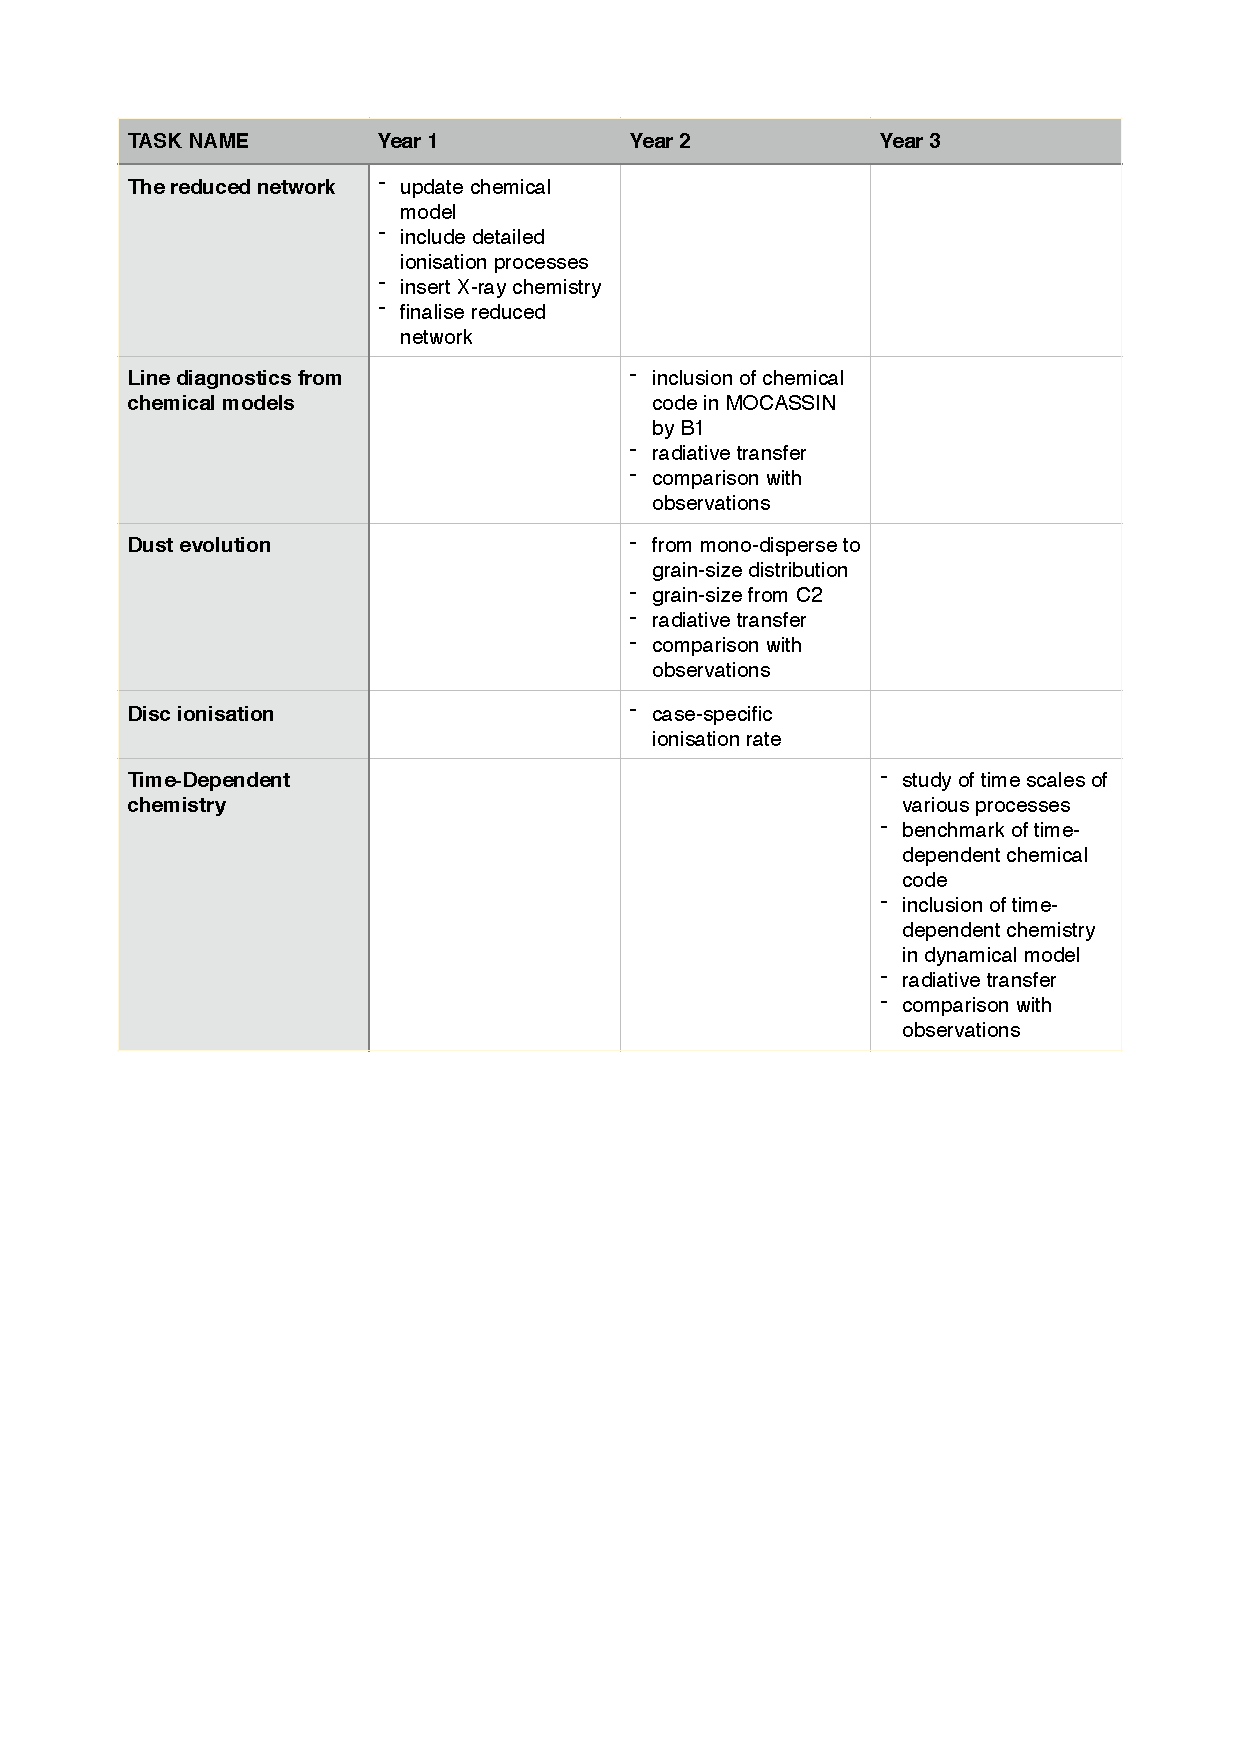
\includegraphics[width=0.9\textwidth]{GanntB2.pdf}
  
   \caption{Gannt chart for B2. More details have been outlined in the previous section.}
              \label{FigGam}
    \end{figure}

{\Tcol\bf Year 1}: (i) focus on the chemical network update, to make sure that all the most recent reaction rates will be included. This will be done by comparing our code with KIDA\footnote{http://kida.obs.u-bordeaux1.fr}, the kinematic database for astrochemistry, as well as with comprehensive literature research.  (ii) Include detailed ionisation processes, taking into account the effects of ionisation-recombination from FUV and CRs. (iii) Include X-ray chemistry based on the extensive literature work available as well work done within the ProDiMo code. (iv) Finalise the reduced chemical network, including Ne and Ar, and test/benchmark it. 

{\Tcol\bf Year 2}: (i) inclusion of reduced chemical network in MOCASSIN-KROME. (ii) Calculation of the chemical-physical model, which will then be used as input in radiative transfer code to produce dust continuum emission and line fluxes. (iii) Comparison with observations and further update of chemical code based on observational constraints. (iv) Study of the effect of changing the grain size from mono-disperse (0.1 $\mu$m) to MRN grain-size distribution (Mathis et al.\ 1977) or evolved-MRN distributions (e.g.\ Zhao et al.\ 2016; Ivlev et al.\ 2016). (v) ionisation level calculations. (vi)  Calculation of an updated chemical-physical model, which will then be used as input in radiative transfer code to produce dust continuum emission and line fluxes. Comparison with observations.

{\Tcol\bf Year 3}: (i) study of time scales of various processes in chemical and dynamical model. (ii) Benchmark of time-dependent reduced chemical code. (iii) Inclusion of time-dependent chemistry in dynamical model. (iv)  Calculation of an updated chemical-physical model, which will then be used as input in radiative transfer code to produce dust continuum emission and line fluxes. Comparison with observations.

{\Tcol\bf Continuous Assessment of New Diagnostics} \connect{Jointly with the B1, C2 and A1 team members as well as with our external collaborators Prof.\ Henning and Prof.\ van Dishoeck, we will regularly compare our models to the observations via the production of synthetic spectra. This will allow us to promptly identify and characterise new wind diagnostics and allow us to use the observations to measure the crucial wind properties of mass loss rate and wind profile, which have a large impact on the formation and evolution of planetary systems.}


\subsection{Data handling}
We will make the sets of line profiles for the different wind and disk characteristics publicly available in electronic format on the public partition of the Research Unit server. The reduced and full networks will also be made available at the end of the first funding period, when they will have reach their final form. 

\subsection{Other information}
% Please use this section for any additional information you feel is
% relevant which has not been provided elsewhere.

Not Applicable 

\subsection{Information on scientific and financial involvement of international cooperation partners}

Not applicable 

\section{Bibliography}

\noindent
Akimkin, V. V. 2015, ARep, 59, 747 \\
Bai, X.-N. 2011a, ApJ, 739, 50 \\
Bai, X.-N. 2011b, ApJ, 739, 51 \\
Balbus, S. A., \& Hawley, J. F. 1991, ApJ, 376, 214 \\
Caselli, P., et al.\ 2002, ApJ, 572, 238 \\
Cleeves, L. I. et al.\ 2013a, ApJ, 772, 5 \\
Cleeves, L. I. et al.\ 2013b, ApJ, 777, 28 \\
Dudorov, A. E., \& Khaibrakhmanov, S. A. 2014, Ap\&SS, 352, 103 \\
Dzyurkevich, N. et al.\ 2013, ApJ, 765, 114 \\
Ercolano, B. et al.\ 2008, ApJ 688, 398 \\
Ercolano, B. et al.\ 2009, ApJ 699, 1639\\
Fujii, Y. I. et al.\ 2011, ApJ, 743, 53 \\
Glassgold, A. E. et al.\ 1997, ApJ, 480, 344 \\
Heinzeller et al.\ 2011, ApJ, 731, 115 \\
Hutschison et al.\ 2016a, MNRAS, 461, 742\\
Hutschison et al.\ 2016b, MNRAS, 463, 272\\ 
Igea, J., \& Glassgold, A. E. 1999, ApJ, 518, 848 \\
Ilgner, M., \& Nelson, R. P. 2006, A\&A, 445, 205 \\
Ivlev, A. V. et al.\ 2016, ArXiv e-prints, arXiv:1607.03701\\ 
Ivlev, A. V. et al.\  2015, ApJ, 812, 135 \\
Larsson, M. et al.\ 2012, RPPh, 75, 066901\\  
Li, H.-B. et al.\ 2014, in Protostars and Planets VI, ed. H. Beuther, R. Klessen, C. Dullemond, \& T. Henning (Tucson, AZ: Univ. Arizona Press), 101-123 \\
Maret, S. et al.\ 2006, Nature, 442, 425 \\ 
Mathis, J. S. et al.\ 1977, ApJ, 217, 425 \\
Mori, S., \& Okuzumi, S. 2016, ApJ, 817, 52 \\ 
Nishi, R. et al.\ 1991, ApJ, 368, 181 \\
Okuzumi, S. 2009, ApJ, 698, 1122 \\
Okuzumi, S. et al.\ 2011a, ApJ, 731, 95 \\
Okuzumi, S. et al.\ 2011b, ApJ, 731, 96 \\
Oppenheimer, M., \& Dalgarno, A. 1974, ApJ, 192, 29 \\
Panoglou, D. et al.\ 2012, A\&A, 538, 2 \\
Salmeron, R., \& Wardle, M. 2008, MNRAS, 388, 1223 \\
Sano, T., Miyama, S. M. et al.\ 2000, ApJ, 543, 486 \\
Semenov, D. et al.\ 2004, A\&A, 417, 93 \\
Turner, N. J. et al.\ 2014, in Protostars and Planets VI, ed. H. Beuther, R. Klessen, C. Dullemond, \& T. Henning (Tucson, AZ: Univ. Arizona Press), 411-432 \\
Umebayashi, T. 1983, PThPh, 69, 480 \\
Umebayashi, T., \& Nakano, T. 1990, MNRAS, 243, 103 \\
Umebayashi, T., \& Nakano, T. 2009, ApJ, 690, 69 \\
Velikhov, E. P. 1959, JETP, 36, 1398 \\
Weingartner, J. C., \& Draine, B. T. 1999, ApJ, 517, 292 \\
Weingartner, J. C., \& Draine, B. T. 2001, ApJS, 134, 263 \\
Weingartner, J. C. et al.\ 2006, ApJ, 645, 1188
Zhao, B. et al.\ 2016, MNRAS, 460, 2015\\

\section{Requested modules/funds}
\renewcommand{\leftmark}{\sc  Requested modules/funds}
% Explain each item for each applicant (stating last name, first name).

\subsection{Basic Module}

\subsubsection{Funding for Staff}
We require funding for one Postdoc to work jointly at the MPE with Prof.\ Caselli and at the LMU in the group of
Prof.\ Ercolano.
A Postdoc with at least some experience of astrochemistry would be certainly desirable  to work on this complex  project. The Postdoc will receive scientific support form the PIs, but also from experienced astrochemists and plasma physicists (e.g.\ Dr.\ Ivlev, Dr.\ Thi) at the Centre for Astrochemical Studies led by Prof.\ Caselli at the MPE. 

In case of an award Dr.\ Sz$\ddot{\textsf u}$cs, currently working at
the MPE in the group of PI Caselli, has expressed interest in taking on the position. His expertise in this field would be very beneficial to the achievement of the aims of this project.

\subsubsection{Direct Project Costs}


\paragraph{Equipment up to EUR 10,000, Software and Consumables}

Theoretical numerical research can only be done when sufficient and
appropriate computational facilities are available. While production
runs will be done on supercomputer facilities, a substantial part of
the work in this project is code development. Testing these codes on
realistic problems requires a workstation for the postdoc
students -- which is beyond the standard base equipment
(Grundausstattung). We therefore request a workstation-grade desktop
computer for the PhD position for \EUR{3 000}.

\paragraph{Travel Expenses}

Total: 17400 \EUR{} Justification : 
Each year one national trip (meeting of Astronomical Society, national
meetings) and one international trip (conference, visit
collaborators) for the postdoc and one PI (Caselli - Note that Ercolano has
placed her travel requests in Project B1). 
During the course of the project 2 one week long visits to our main
international collaborator, Dr T. Grassi (Copenhagen). 

Cost estimate: 
\begin{itemize}
\item National trip: 5 overnight stays, train/airfare,
conference fee; 1000 \EUR{} (6000 in total over 3 years).
\item International trip: 6 overnight stays, airfare, conference fee;
  1500 \EUR{} (9000 total over 3 years).
\item Visit to/from J. Owen: airfare, 6 overnight stay 1200 \EUR{} (2400
  for 2 visits)
\end{itemize}


%\paragraph{Visiting Researchers (excluding Mercator Fellows)}

%Not Relevant 


%\paragraph{Other Costs}

%None

\paragraph{Project-related publication expenses}

We request 750 \EUR{}/year (total 2250 \EUR{}) for publication expenses.

%\subsubsection{Instrumentation}

%None 

%\paragraph{Equipment exceeding EUR 10,000} 

%None

%\paragraph{Major Instrumentation exceeding EUR 100,000} 

%None

% \subsection{Module Temporary Position}
% 
% Not Relevant
% 
% \subsection{Module Replacement Funding}
% 
% Not Relevant
% 
% \subsection{Module Mercator Fellows}
% 
% Not Relevant
% 
% \subsection{Module Public Relations Funding}
% 
% Not Relevant

\section{Project requirements}
\renewcommand{\leftmark}{\sc Project requirements}

\subsection{Employment status information}
% For each applicant, state the last name, first name, and employment
% status (including duration of contract and funding body, if on a
% fixed-term contract).

Paola Caselli, Director at the Max Planck Institute for Extraterrestrial Physics (MPE) -- permanent 

Barbara Ercolano, Professor at the Ludwig-Maximilians-Universit\"at
M\"unchen -- permanent

%\subsection{First-time proposal data}
% Only if applicable: Last name, first name of first-time applicant.

%Not Relevant

\subsection{Composition of the project group}
% List only those individuals who will work on the project but will not
% be paid out of the project funds. State each personテ「竄ャ邃「s name, academic
% title, employment status, and type of funding.

Alexei Ivlev, Dr, permanent scientist at the MPE 
Wing Fai, Thi, Dr, postdoctoral assistant at the MPE

\subsection{Cooperation with other researchers}

\subsubsection{Planned cooperation on this project}

\paragraph{Collaborating researchers for this project within the
  Research Unit}
%Each proposal must be accompanied by a description of how the project
%is integral to the Research Unit, %both in terms of subject matter
%and organisation. This includes a description of the cooperation with
%%others participating within the Research Unit. 

\connect{This project is intimately linked to project B1 (PI Ercolano) and to project C2 (PI Ercolano). 
It requires the input from the radiation-hydrodynamic models from B1 as well as the MOCASSIN-KROME code which is developed by the PI Ercolano for B1 and B2 (with different immediate objectives). It also requires input from project C2 (PI Ercolano) and will work closely with T. Birnstiel (C1, C2) for help in the implementation of the dust models. The irradiating
  spectra used for the models will be obtained in co-operation with
  the team of project A2.  The synthetic spectra will be compared with observations with the help of the A1 team (PI Testi) and our external collaborators Prof.\ Henning and Prof.\ van Dishoeck. }

\connect{This can also provide the final machinery to projects D1
  and D2 to calculate the chemical abundance of molecules. These can
  then be used for line transfer calculations, which are essential to
  probe the gas and the kinematics of Type 2 TDs.}

\paragraph{Collaborating researchers for this project outside of
  the Research Unit}

Dr.\ Grassi, the author of the KROME package has already helped Prof.\ Ercolano with the implementation of KROME into MOCASSIN and is expected to help further in implementing the new networks and optimising the chemistry routine (inclusion, for example, of a better equilibrium chemistry option. 
It is envisioned that Dr.\ Grassi will play regular visits to our group.    

\subsubsection{Researchers with whom you have collaborated scientifically within the past three years}
% This information is important for DFG to exclude possible conflicts of interest.
% Please mention not only the names of the cooperation partners but also their institution and city.
% Scientists already mentioned in the previous two subsubsections do not have to be mentioned
% again.

Maite Bertran (INAF-Osservatorio Astrofisico di Arcetri), Aaron Boley (University of British Columbia), Sandra Brünken (University of Cologne), Stephanie Cazaux (University of Groningen), Cecilia Ceccarelli (Univ. Grenoble Alpes), Francesco Fontani (INAF-Osservatorio Astrofisico di Arcetri), Thomas Hartquist (University of Leeds), Izaskun Jimenez-Serra (Queen Mary University London), Eric Keto (Harvard-Smithsonian Center for Astrophysics), Marco Spaans (University of Groningen), Jonathan Tan (University of Florida), Stephan Schlemmer (University of Cologne), Charlotte Vastel (Université de Tulouse), Malcolm Walmsley (INAF-Osservatorio Astrofisico di Arcetri)
 Niederhofer (STSci, USA); M. Hilker (ESO, Garching); N. Bastian (U. Liverpool,
UK); M. Guarcello (U. Palermo, Italy); M. Tazzari (U. Cambridge, UK);
A. Natta (Florence, Italy); R. Alexander (U. Leicester); D. Hubber
(LMU); J. Dale (U. Hertfordshire, UK); C. Koepferl (LMU); I. Bonnell
(U. St. Andrews, UK); A. McLeod (ESO, Garching); D. Boneberg
(U. Cambridge, UK); R. Parker (U. Liverpool, UK); R. Wesson (UCL,
London, UK); M. Barlow (UCL, London, UK); A. Glassgold (u. Berkeley,
USA); C. Manara (ESA, Noordwjik, Netherlands); A. Danekhar (CfA,
Harward, USA); Q. Parker (Sidney, Australia); S. Casassus
(U. de Chile, Santiago, Chile); I. Pascucci (U. Arizona, USA);
A. Bevan (UCL, London, UK).

\subsection{Scientific equipment}
% List larger instruments that will be available to you for the
% project. These may include large computer facilities if computing
% capacity will be needed. 

The CAS centre led by Prof.\ Caselli has available computer facilities for visiting scientists and students. CAS has its own cluster: an HPC cluster comprising of 25 nodes with 20 cores and 128 GB memory each; 4 nodes with 20 cores and 256 GB memory each (Infiniband, 50 TB storage, Login-Node, Batch-System; 2 Compute nodes, i.e.\ 2 nodes with 20 cores and 512 GB (10 TB storage). 


The group of Prof.\ Ercolano has two own computer clusters comprising 

\begin{itemize}
\item 2 CPU Intel Xeon X5650 (Westmere, beginning
2010, 2.66 GHz) 6 cores each 12 cores total (24 virtual) 74 GB ram.

\item 4 CPU Intel Xeon E7-4850 (Ivy Bridge, beginning 2014, 2.30 GHz)
12 cores each 48 cores total (96 virtual) 660 GB ram.

\end{itemize}

Further computational power is provided through the C2PAP facility of the Excellence Cluster to which
the group has guaranteed time. This comprises 126 nodes, each node with 2 CPU Intel Xeon E5-2680 (Sandy
Bridge, beginning 2012, 2.7 GHz) 8 cores each 16 cores total (32
virtual) 64 GB ram. Note that while the future of the Excellence
Cluster Universe is uncertain, the C2PAP facilities will be in any
case supported by the LMU. 

The facilities at the Leibniz Rechenzentrum (LRZ) , with the iDataPlex
HPC System HYDRA with Intel Ivy Bridge processors (~3500 nodes with 20
cores at 2.8 GHz each are also available to us.

%\subsection{Project-relevant interests in commercial enterprises}
% Information on connections between the project and the production
% branch of the enterprise.

%Not Relevant


%\subsection{Additional information}
% If applicable, please list proposals requesting major
% instrumentation and/or those previously submitted to a third party
% here.

%Not Relevant


\end{document}
